\setlength{\textfloatsep}{0pt}% Remove \textfloatsep


\begin{algorithm}[htpb]

\caption{\compas: A {\bf Com}munity {\bf P}reserving Sampling {\bf A}lgorithm for {\bf S}treaming Graph}\label{alg:compas}
\KwData{$S$: Graph stream, $n$: Sample size,  $\alpha$: Initial fraction of nodes inserted,  $\beta$: Edge density threshold, $n_d$: size of the buffer, $Algo$: a community detection algorithm}\label{algo_compas}
\KwResult{Sampled Subgraph $G_s(V_s, E_s)$, $C_s$}
Initialize $G_s$: $V_s=\phi$, $E_s=\phi$\\
Crate an empty buffer $\mathcal{H}$ of size $n_d$\\
Initialize buffer $\mathcal{H}$: $\mathcal{H}_c=\phi$, $\mathcal{H}_p=\phi$\\
$flag=1$, $t=0$\\
\For{$e_t$ in the graph stream $S$}{
$e_t=\{u,v\}$\\
%\If{$|V_s|\neq n$}{
\If{$\frac{|V_s|}{n}<\alpha \wedge e_t\notin E_t$}{\label{b:step1}
$V_s=V_s\cup u \cup v$\\
$E_s=E_s\cup e_t$\\
\textbf{Continue;}\label{e:step1}
}
\ElseIf{flag==1}{
Run $Algo$ on $G_s$ and detect community structure $C_s$\label{algo} \\
$flag$=0\\
}
\ElseIf{$u, v\in V_s$}{
$V_s,E_s,C_s=BothinSample(u,v,e_t,V_s,E_s,C_s)$\\
}
\ElseIf{$u\in V_s \wedge v\notin V_s \wedge v\notin \mathcal{H}$}{
$V_s,E_s,C_s,\mathcal{H}=OneinSampleOneNew(u,v,e_t,V_s,E_s,\mathcal{H},C_s)$
}
\ElseIf{$u \in V_s \wedge v\notin V_s \wedge v\in \mathcal{H}$}{
$V_s,E_s,C_s,\mathcal{H}=OneinSampleOneinBuffer(u,v,e_t,V_s,E_s,\mathcal{H},C_s)$
}
\ElseIf{$u\notin V_s \wedge u\in \mathcal{H} \wedge v\notin V_s \wedge v\notin \mathcal{H}$}{
$V_s,E_s,C_s,\mathcal{H}=OneinBufferOneNew(u,v,e_t,V_s,E_s,\mathcal{H},C_s)$
}
%\ElseIf{$u,v\notin V_s \wedge u,v\in \mathcal{H}$}{
%$\mathcal{H}_c[u]=\mathcal{H}_c[u]+1$\\
%$\mathcal{H}_c[v]=\mathcal{H}_c[u]+1$
%}
\ElseIf{$u,v\notin V_s \wedge u,v\notin \mathcal{H}$}{
$V_s,E_s,C_s,\mathcal{H}=BothNew(u,v,e_t,V_s,E_s,\mathcal{H},C_s)$
}
\ElseIf{$u,v\notin V_s \wedge u,v\in \mathcal{H}$}{
$\mathcal{H}=BothinBuffer(u,v,\mathcal{H})$
}
$t=t+1$
}

%}
\Return $G_s$, $C_s$
\end{algorithm}



\vspace{10mm}

\section{Proposed Algorithm: COMPAS}
\label{algorithm}

Here we propose \compas, a {\bf Com}munity {\bf P}reserving sampling {\bf A}lgorithm for {\bf S}treaming graphs.
\compas~aims at sampling a streaming graph in such a way that its underlying community structure is preserved in the sample (a pseudo-code and a toy example are presented in Algorithm~\ref{algo_compas} and Figure~\ref{fig_algo} respectively). To start with, \compas~keeps on adding streaming edges (nodes) into the sample $G_s$ as long as a certain fraction of nodes $\alpha$ is inserted (lines \ref{b:step1}-\ref{e:step1}). This in turn provides an initial knowledge about the graph structure. Once the threshold is reached, a pre-selected community detection algorithm $Algo$ is run on $G_s$ to detect the initial community structure (line \ref{algo}). After that, it interweaves both graph sampling and community detection in such a way that each task gets benefits from the other. Once an edge $e_t$ is taken from the stream, \compas~ judiciously inserts $e_t$ into $G_s$ with the help of a buffer $\mathcal{H}$ which is composed of $\mathcal{H}_c$ and $\mathcal{H}_p$. $\mathcal{H}_c$ counts the ``number of hits'' of a node (i.e., number of times a node is encountered till that time)\footnote{In streaming graph, an edge might appear multiple times.}, and $\mathcal{H}_p$ keeps track of the current parent of a node (i.e., node with which it arrived last). \iffalse{} \TODO{This is not clear. How do you decide which node is the ``current'' parent of another node in a graph?}\fi A streaming edge $e_t=\{u,v\}$ is first inserted into  $\mathcal{H}$, and depending upon the current position of $u$ and $v$ (whether in the buffer or in the sample), their counts in $\mathcal{H}_c$, their current parents in $\mathcal{H}_p$, and the current community structure $C_s$ of $G_s$, a decision that which node/edge is to be inserted into $G_s$ is taken. One of the six different submodules is invoked to systematically handle this decision.
%In order to maintain non-redundancy inside a community, \compas~never allows an existing  community to cross a certain edge density threshold $\beta$. 
Throughout the iterations, \compas~maximizes {\em modularity} \cite{newman2004analysis}, a well-studied objective function for community detection defined below:
\begin{equation}\label{modularity}\small
Q(G(V,E),C)=\sum_{c\in C} (\frac{m_c}{M} - \frac{D_c^2}{4M^2})
\end{equation}
where $C$ is the community structure of $G$, $m_c$ is the total number of edges inside $c$, $D_c$ is the sum of degree of all the nodes inside a community $c\in C$, and $M=|E|$ is the total number of edges $G$. In this section, we individually present each submodule of \compas~in details.

Once the initial threshold $\alpha$ is reached, a community finding algorithm $Algo$ is used to detect the initial community structure of $G_s$ (denoted as $C_s$) (line 12). Then in every occurrence of a new edge $e_t=\{u,v\}$, it is not allowed to enter into the sample immediately; instead depending upon the current position of $u$ and $v$ different subroutines are invoked  
to place the edge (i.e., two end nodes) into the buffer. This in turn may remove an existing node out of the buffer and connect it with its parent in $G_s$. $C_s$ is adjusted accordingly. 
In this section, we describe different subroutines in details.





\noindent\textbf{(i) \underline{Both $u$ and $v$ are present in the sample:}} When both $u,v$ are in $V_s$, $BothinSample()$ (see Function 1) is called from line 15 of Algorithm \ref{algo_compas}.  We further divide this case into two subcases: $e_t$ is an intra-community edge (totally inside a single community) or an inter-community edge (connecting two communities $C(u)$ and $C(v)$). In the former case (edge $\{b,d\}$  in Figure~\ref{fig_algo}), addition of $e_t$ will strengthen the internal community structure according to Proposition~\ref{1}\footnote{Detailed proofs of all the propositions can be found in \cite{si}.}. We also know from Proposition~\ref{2} that adding an intra-community edge should not split the current community. Therefore we leave $C_s$ in its current form without any modification.

In case of $e_t$ connecting two different communities (edge $\{b,f\}$ in Figure \ref{fig_algo}), several possibilities may arise. $u$ (or $v$) may leave its current community and join in other community. Additionally, if the community membership of $u$ (or $v$) is changed, it can also pull out its neighbors to join with it, and some of the neighbors might eventually want to change their memberships as well. According to Proposition~\ref{3}, we know that if $u$ (or $v$) ever changes its community membership, $C(v)$ (or $C(u)$) would be the best new community for it. But how do we quickly decide it? Here we provide a criteria to check the change in membership for $u$ and $v$ in Proposition~\ref{complex}. If both $\Delta Q(u,C(u),C(v))$ and $\Delta Q(v,C(v),C(u))$ (where $\Delta Q(u,C(u),C(v))$ indicates the change in modularity after assigning $u$ from $C(u)$ to $C(v)$) fail to satisfy the criteria (see Corollary 1), we can retain the current community structure. Otherwise, we move $u$ (or $v$) to $C(v)$ (or $C(u)$) and consequently we let its neighbors decide their best move in the similar way. 


\begin{figure}[!t]
\centering
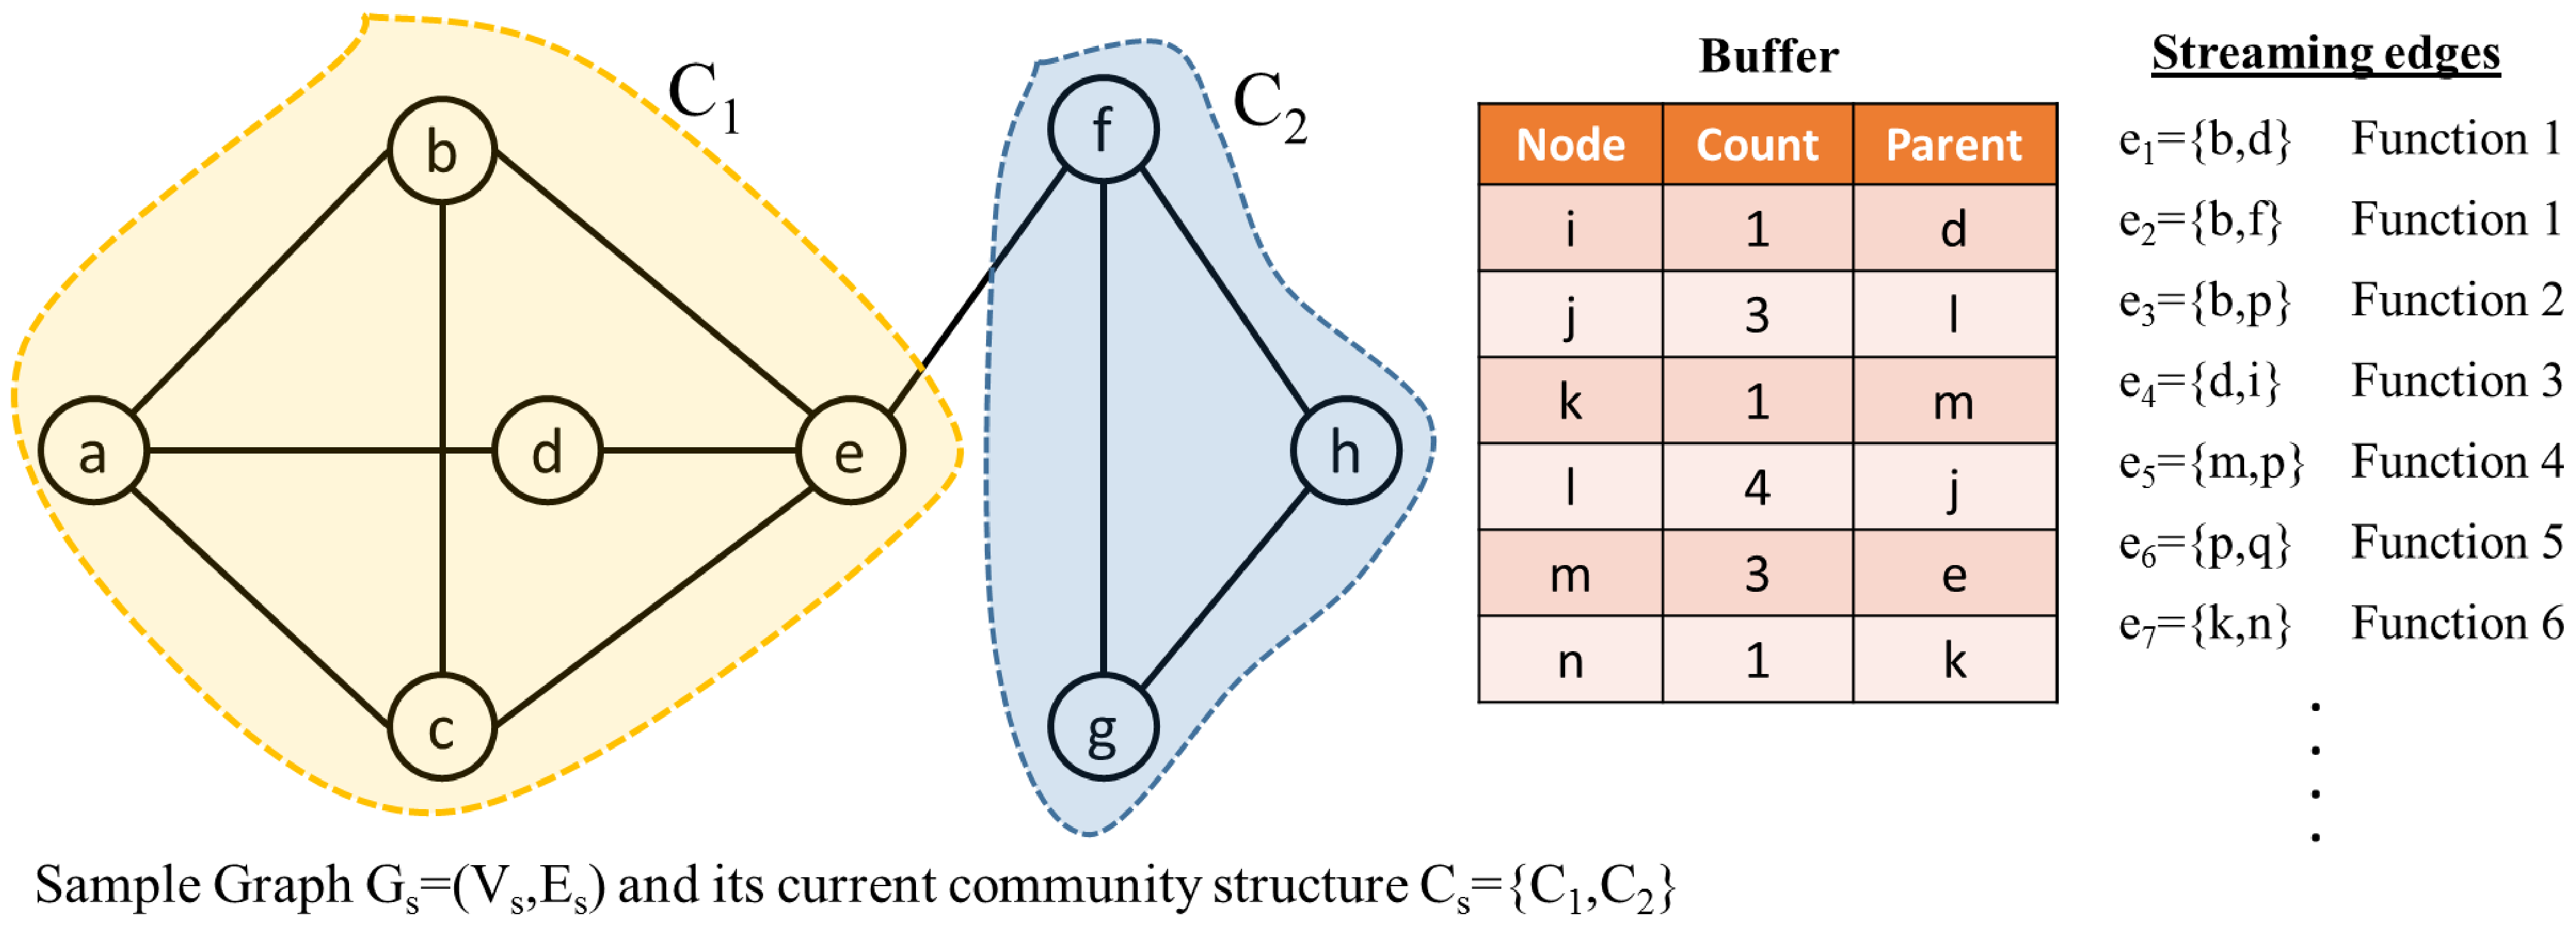
\includegraphics[width=\columnwidth]{./texfiles/Chapter_2/figures/demo.eps}
%\vspace{-5mm}
\caption{Toy example depicting various conditions handled by \compas~ when a streaming edge arrives.}\label{fig_algo} 
%\vspace{-3mm}
\end{figure}

\begin{prop}\label{1}
For a community $c\in C$, if $D_c\leq M-1$ $($where $M=|E|)$ then addition of an edge within $c$ will increase its modularity.
%\vspace{-2mm}
\end{prop}


\begin{proof}
From Equation \ref{modularity}, we see the contribution of individual community $c\in C$ in modularity as: $Q_c=\frac{m_c}{M} - \frac{D_c^2}{4M^2}$. 
%where $m_c$ is the number of edges inside $c$, $M$ is the total number of edges in the graph, and $D_c$ is the sum of degrees of all the nodes in $c$. 

Addition of a new edge within $c$, the $c$'s contribution of modularity becomes:
\[
Q'_c=\frac{m_c+1}{M+1} - \frac{(D_c+2)^2}{4(M+1)^2}
\]

So the increase in modularity is $\Delta Q_c=Q'_c-Q_c$,
\[
\begin{split}
\Delta Q_c=&\frac{4M^2-4m_cM^2-4D_cM^2-4m_cM+2D_c^2M+D_c^2}{4(M+1)^2M^2}\\
&\geq \frac{4M^2-6D_cM^2-2D_cM+2D_c^2M+D_c^2}{4(M+1)^2M^2}\\
&\geq\frac{(2M^2-2D_cM-D_c)(2M-D_c)}{4(M+1)^2M^2}\\
&\geq 0
\end{split}
\]
The equality holds if $D_c\leq M-1$. This thus implies $(2M^2-2D_cM-D_c)\geq 0$. This proves the proposition.
\end{proof}



\begin{prop}\label{2}
For a community $c\in C$, addition of any intra-community edge into $c$ should not split it into smaller communities.
%\vspace{-2mm}
\end{prop}




\begin{proof}
We will prove this proposition by contradiction.
Assume that once a new intra-community edge is added into $c$, it gets split into $k$ small modules, namely $X_1$, $X_2$, $\cdot$,$X_k$. Let $D_{X_i}$ and $e_{ij}$ be the total degree of nodes inside $X_i$ and number of edges connecting $X_i$ and $X_j$ respectively. 


Recall that the contribution of $X_i$ in the modularity value is $Q_{X_i}=\frac{m_{X_i}}{M} - \frac{D_{X_i}^2}{4M^2}$.  
Before adding the edge, we have $Q_c \geq \sum_{i=1}^k Q_{X_i}$ (where $Q_c$ is the total modularity of community $c$), because otherwise all $X_i$s can be split earlier, which is not in this case. This implies that: $\frac{m_c}{M}- \frac{D_c^2}{4M^2} > \sum_{i=1}^k (\frac{m_{X_i}}{M} - \frac{D_{X_i}^2}{4M^2})$. Since $X_1,X_2,\cdot,X_k$ are all disjoint modules of $c$, $D_c=\sum_{i=1}^k D_{X_i}$ and $m_c=\sum_{i=1}^k m_{X_i} + \sum_{i<j} e_{ij}$. This further implies that:
\[ \frac{m_c}{M}-\sum_{i=1}^k \frac{m_{X_i}}{M} > \frac{D_c^2}{4M^2}- \sum_{i=1}^k \frac{D_{X_i}^2}{4M^2}\]
or,
$\sum_{i<j} e_{ij} > \frac{\sum_{i<j} D_{X_i}D_{X_j}}{2M}
$.
 
 Without loss of generality, let us assume that the new edge is added inside $X_1$. 
Since we assume that after adding the new edge into $c$, it gets split into $k$ small modules, the modularity value should increase because of the split. Therefore, %Therefore, the new modularity $Q'_c<\sum_{i=1}^k Q_{X_i}$. 
This implies that
\[
\begin{split}
& Q'_c < \sum_{i=1}^k Q_{X_i}\\
& \Leftrightarrow \frac{\sum_{i=1}^k m_{X_i} + \sum_{i<j} e_{ij} + 1}{M+1} - \frac{(\sum_{i=1}^k D_{X_i +2})^2}{4(M+1)^2}\\
%& <  \frac{m_{X_1}+1}{M+1} - \frac{(D_{X_1}+2)^2}{4(M+1)^2}  + \sum_{i=2}^k  (\frac{m_{X_i}}{M+1} - \frac{D_{X_i}^2}{4(M+1)^2} )\\
%&\Leftrightarrow \frac{\sum_{i=1}^k m_{X_i} + \sum_{i<j} e_{ij} + 1}{M+1} - \frac{(\sum_{i=1}^k D_{X_i +2})^2}{4(M+1)^2}\\
& < \frac{\sum_{i=1}^k m_{X_i}+1}{M+1} - \frac{(D_{X_1}+2)^2}{4(M+1)^2} - \sum_{i=2}^k \frac{D_{X_i}^2}{4(M+1)^2}\\
&\Leftrightarrow \sum_{i<i} e_{ij} < \frac{\sum_{i=1}^k D_{X_i} - 2 D_{X_1} + \sum_{i<j} D_{X_i}D_{X_j}}{2(M+1)}
\end{split}
\]
Since $\sum_{i=1}^k D_{X_i} - 2D_{X_1} < 2M$, this implies that 
\[
\begin{split}
\frac{\sum_{i<j}D_{X_i}D_{X_j}}{2M}  < \sum_{i<j}e_{ij} 
&< \frac{\sum_{i=1}^k D_{X_i} - 2D_{X_1} + \sum_{i\neq j}{D_{X_i}D_{X_j}}}{2(M+1)}\\
& <\frac{\sum_{i<j}D_{X_i}D_{X_j}}{2M}+1
\end{split}
\]
Therefore, the proposition holds.
\end{proof}









\begin{prop}\label{3}
If a new edge $(u,v)$ connecting two communities $C(u)$ and $C(v)$ is introduced, $C(u)$ $($or $C(v))$ is the best candidate for $v$ (or $u$) if it should ever change its membership.
%\vspace{-2mm}
\end{prop}


\begin{proof}
The method is inspired by \cite{PhysRevE.78.046115} that a vertex $u$ is influenced by two factors: $F^c_{in}(u)$ the force that keeps $u$ stay in its own community $c$, and $F^c_{out}(u)$, the force that a community $S$ imposes to $u$ in order to bring $u$ to $S$ as follows:
\[
F^c_{in}(u)=e_c^u-\frac{d_u(D_c-d_u)}{2M}
\]
and 
\[
F^S_{out}(u)=max_{S\in NC(u)} \{e_S^u - \frac{d_u D_{outS}}{2M}\}
\]
where $NC(u)$ is the set of neighboring communities of $u$, and $D_{outS}$ is the total degree of vertices outside $S$.

Now we will show that the presence of new edge $(u,v)$ will strengthen $F^{C(v)}_{out}(u)$ and weaken $F^S_{out}(u)$. In other words, we will show that $F^{C(v)}_{out}(u)$ increases while $F^S_{out}(u)$ decreases for all $S \in C \wedge S \notin \{C(u),C(v)\}$.
\[
\begin{split}
&F^{C(v)}_{out}(u)|_{new} - F^{C(v)}_{out}(u)|_{old}\\
&=(e_u^{C(v)}+1-\frac{(d_u+1)(d_{outC(v)}+1)}{2(M+1)} - (e_u^{C(v)} - \frac{d_ud_{outC(v)}}{2M})\\
&= \frac{2M+d_ud_{outC(v)}}{2(M+1)} - \frac{d_ud_{outC(v)}+d_{outD(v)}+d_u+1}{2(M+1)}\\
&\geq \frac{2M+d_ud_{outC(v)}}{2(M+1)} - \frac{d_u d_{outC(v)}+d_{outC(v)}+d_u+1}{2(M+1)}\\
&>0
\end{split}
\]
Therefore $F^{C(v)}_{out}(u)$ is strengthened when a new edge $(u,v)$ is introduced. Further, for any community $S\in C \wedge S\notin \{C(u),C(v)\}$
\[
\begin{split}
& F^{S}_{out}(u)|_{new} - F^{S}_{out}(u)|_{old}\\
&= (e^S_u-\frac{(d_u+1)d_{outS}}{2(M+1)}) - (e^S_u - \frac{d_ud_{outS}}{2M})\\
&= d_{outS}(\frac{d_u}{2M} - \frac{d_u+1}{2(M+1)})<0
\end{split}
\]

This implies that $F^S_{out}(u)$ is weakened when $(u,v)$ is added. Therefore,  the proposition holds.
\end{proof}




\begin{prop}\label{complex}
If a new edge $(u,v)$ is added into the graph, then joining $u$ to $v$'s  community $C(v)$ will increase the modularity value  if $\Delta Q(u,C(u),C(v)) \equiv 4(M+1)(e_{C(v)}^u+1-e_{C(u)}^u)+e_{C(v)}^u(2D_{C(v)}-2d_u-e_{C(u)}^u) - 2(d_u+1)(d_u+1+d_{C(v)}-d_{C(u)})>0$.
%\vspace{-2mm}
\end{prop}


\begin{proof}
Vertex $u$ will leave its current community $C(u)$ and join $v$'s community $C(v)$ if
\[
\begin{split}
& Q_{C(v)+u} + Q_{C(u)-u} > Q_{c(u)} + Q_{C(v)}\\
&\Leftrightarrow \frac{m_{C(v)}+e_{C(v)}+1}{M+1} - \frac{(d_{C(v)}+d_u+2)^2}{4(M+1)^2}+\\
&\frac{m_{C(u)} - e_{C(u)}}{M+1} - \frac{(d_{C(u)}-d_u-e_{C(u)})}{4(M+1)^2} \\
& > \frac{m_{C(v)}}{M+1} - \frac{(d_{C(v)}+d_u+2)^2}{4(M+1)^2} + \frac{m_{C(u)}}{M+1} - \frac{(d_{C(u)}+1)^2}{4(M+1)^2}\\
&\Leftrightarrow 4(M+1)(e_{C(v)} +1 -e_{C(u)}) + e_{C(u)}(2d_{C(v)} - 2d_{C(u)}-e_{C(u)})\\
& - 2(d_{C(u)}+1)(d_{C(u)}+1+d_{C(v)}-d_{C(u)})>0
\end{split}\]
\end{proof}


\noindent{\bf Corollary 1.} {\em If the condition in Proposition \ref{complex} is not satisfied, then neither $u$ nor its neighbors should be assigned to $C(v)$.}


%\vspace{-3mm}
\begin{function1}[!h]
\caption{$BothinSample(u,v,e_t,V_s,E_s,C_s)$ \iffalse\TODO{Notation mismatch. Are $\Delta_{u,C_s(u),C_s(v)}$ and $\Delta Q(u, C_s(u),C_s(v))$ the same?} \textcolor{blue}{corrected}\fi} 
\If{$C_s(u)==C_s(v)$}{
$E_s=E_s\cup e_t$
}
\Else{
\If{$\Delta Q (u,C_s(u),C_s(v))<0 \wedge \Delta Q (v,C_s(v),C_s(u))<0$}{
\Return{$V_s,E_s,C_s$}}
\Else{
$w\leftarrow arg max \{\Delta  Q(u,C_s(u),C_s(v)),\Delta Q(v,C_s(v),C_s(u))\}$\\
Move $w$ to a new community and update $C_S$\\
\For{$t\in N(w)$}{
Let $t$ decide its own community\\
Update $C_s$
}
}
}
\Return $V_s,E_s,C_s$   
\end{function1}

%\vspace{-3mm}
\noindent\textbf{(ii) \underline{$u$ is in sample and $v$ is new:}} When a new node $v$  connecting node $u\in G_s$ appears, $OneinSampleOneNew()$ (see Function 2) is called from line 17 of Algorithm 1 (edge $\{b,p\}$ in Figure \ref{fig_algo}). In this case, we do not add $\{u,v\}$ into the sample immediately. Instead, we first insert $v$ into $\mathcal{H}$ if $\mathcal{H}$ is not full. If $\mathcal{H}$ is full, we pick one node $x$ from $\mathcal{H}$ preferentially based on $\mathcal{H}_c[x]$ with an additional constraint that $\mathcal{P}(x)$, the parent of $x$  should be in $G_s$\footnote{The additional constraint allows to avoid a disconnected component being created in the sample.} (for example, in Figure~\ref{fig_algo} if the buffer is full although node $l$ has highest count we do not pick $l$ from the buffer  because its parent node $i$ is not in $G_s$; instead we pick $m$ which satisfies both the constraints).  $x$ is then added to $G_s$ through the edge $\{\mathcal{P}(x),x\}$ (line 10 in Function 2) and is assigned the community of $\mathcal{P}(x)$ (line 11 in Function 2). We also check if including $x$ in $G_s$ violates the sample size constraint through the function 
%If $G_s$ is already full (i.e., $V_s=n$) then 
$CheckResizeSample()$ (Function 7). If $G_s$ is already full (i.e., $V_s=n$), one existing node which has lowest degree is removed from $G_s$ and the community structure is adjusted accordingly using $CommunityAfterNodeRemoval()$ (both Functions 7 and 8 are discussed later).

%If $\mathcal{H}$ is full, we will remove one node $x$ from $\mathcal{H}$ preferentially based on the  number of times $x$ is encountered previously and add it into $G_s$. To do so, we first check if $P(x)$, the parent of $x$ is already in $G_s$; if exists then we assign $x$ into the community of $P(x)$ (line 11 of Function 2). We also check if assigning $x$ into $G_s$ will not violate the size of $G_s$. If $G_s$ is already full (i.e., $V_s$=n) then we call $CheckResizeSample()$ (Function 6) which will remove  from $G_s$ one existing node which has lowest degree and adjust the community accordingly using $CommunityAfterNodeRemoval()$ (discussed later in Function 7). On the other hand, if $P(x)$ is not in $G_s$ but in $\mathcal{H}$, we remove both $x$ and $P(x)$ from $\mathcal{H}$ and add them into $G_s$. Once again, if $G_s$ is full, two nodes are removed from $G_s$ based on the lowest degree as mentioned earlier and communities are adjusted (line 18 in Function 2). Then a new community is created, and $x$ and $P(x)$ are added into it (line 22 in Function 2).




%\vspace{-3mm}

\begin{function2}[!t]
\caption{$OneinSampleOneNew(u,v,e_t,V_s,E_s,\mathcal{H},C_s)$}
\If{$\mathcal{H}$ is not full}{
Insert $v$ to $\mathcal{H}$\\
}
\Else{
Choose a node $x$ with $\mathcal{P}(x) \in V_s$ from $\mathcal{H}$ preferentially based on $\mathcal{H}_c$\\
Remove $x$ from $\mathcal{H}$\\
$\mathcal{H}_c[x]=0$\\
$\mathcal{H}_p[x]=\phi$\\
$V_s,E_s,C_s = CheckResizeSample(V_s,C_s,n,1)$\\
$V_s=V_s\cup x$\\
$E_s=E_s\cup \{P(x),x\}$\\
$C_s(x)=C_s(P(x))$\\
Update $C_s$\\ %\TODO{Not clear what this line does. I do not see a separate update function.}\\
Insert $v$ to $\mathcal{H}$\\
}

$\mathcal{H}_c[v]=1$\\ 
$\mathcal{H}_p[v]=u$\\ 
\Return $V_s,E_s,C_s,\mathcal{H}$   
\end{function2}

%\vspace{-3mm}
\noindent\textbf{(iii) \underline{$u$ is in sample and $v$ is in buffer:}} In this case (edge $\{d,i\}$ in Figure \ref{fig_algo}), $OneinSampleOneinBuffer()$ (see Function 3) is called from line 19 of Algorithm 1. We first check the sample size constraint (line 4 in Function 3) and accordingly add $v$ (and edge $\{u,v\}$) into $G_s$. $v$ is further assigned to $C(u)$.

%\vspace{-3mm}
\begin{function3}[!h]
\caption{$OneinSampleOneinBuffer(u,v,e_t,V_s,E_s,\mathcal{H},C_s)$}
Remove $v$ from $\mathcal{H}$\\
$\mathcal{H}_c[v]=0$\\
$\mathcal{H}_p[v]=\phi$\\
$V_s,E_s,C_s = CheckResizeSample(V_s,C_s,n,1)$ \\
$V_s=V_s\cup v$\\
$E_s=E_s \cup \{ v,\mathcal{P}(v)\}$\\
%\If{$V_s == n$}{
%Remove one nodes (and all adjacent edges) from $G_s$ having lowest degree \\
%$C_s=CommunityAfterNodeRemove()$;
%}
$C_s(v)=C_s(u)$\\
Update $C_s$ \\
%\TODO{Not clear what this line does. I do not see a separate update function.}\\
\Return $V_s,E_s,C_s,\mathcal{H}$   
\end{function3}

%\vspace{-3mm}
\noindent\textbf{(iv) \underline{$u$ is in buffer and $v$ is new:}} This case (edge $\{m,p\}$ in Figure \ref{fig_algo}, see Function 4) is similar to Function 2. We first increment the counter corresponding to $u$ in the buffer and add $v$ into the buffer in the same way as mentioned in Function 2.
\vspace{-3mm}
\begin{function4}[!h]
\caption{$OneinBufferOneNew(u,v,e_t,V_s,E_s,\mathcal{H},C_s)$}
$\mathcal{H}_c[u]=\mathcal{H}_c[u]+1$\\
$V_s,E_s,C_s,\mathcal{H} = OneinSampleOneNew(u,v,e_t,V_s,E_s,\mathcal{H},C_s)$\\
\Return $V_s,E_s,C_s,\mathcal{H}$  %\TODO{Check. I think we do not need this line as it is included already in the previous function.{\color{blue}Done}}
\end{function4}
%\vspace{-3mm}

\noindent\textbf{(v) \underline{Both $u$ and $v$ are new:}}
When both $u$ and $v$ are new (edge $\{p,q\}$ in Figure \ref{fig_algo}), $BothNew()$ (see Function 5) is called from line 23 of Algorithm 1. We initially check whether buffer $\mathcal{H}$ is full or not. In case it is not full, we insert $u$ in $\mathcal{H}$ and then call Function 2. Otherwise, we preferentially remove $x$ and $y$ from $\mathcal{H}$ based on the counts in $\mathcal{H}_c$ with the additional constraint that both $\mathcal{P}(x)$ and $\mathcal{P}(y)$ are in $G_s$, and add nodes $x$, $y$ and edges $\{\mathcal{P}(x)$,$x$\}, $\{\mathcal{P}(y)$,$y\}$ into $G_s$. $x$ and $y$ are also assigned to the community of the their respective parents. Finally, $u$ and $v$ are inserted into $\mathcal{H}$. If during the insertion into $G_s$ the sample size is violated, the required number of nodes along with their adjacent edges are deleted from $G_s$ using $CheckResizeSample()$.


%\vspace{-3mm}
\begin{function5}[!t]
\caption{$BothNew(u,v,e_t,V_s,E_s,\mathcal{H},C_s)$}
\If{$\mathcal{H}$ is not full}{
Insert $u$ to $\mathcal{H}$\\
$\mathcal{H}_p[u] = v$\\
$\mathcal{H}_c[u] = 1$\\
$V_s,E_s,C_s,\mathcal{H}= OneinSampleOneNew(u,v,e_t,V_s,E_s,\mathcal{H},C_s)$\\
}
\Else{
Choose nodes $x$, $y$ with $\mathcal{P}(x), \mathcal{P}(y) \in V_s$ \iffalse\TODO{Not $\mathcal{P}(y) \in V_s$?}\textcolor{blue}{corrected}\fi from $\mathcal{H}$ preferentially based on $\mathcal{H}_c$\\
Remove $x$, $y$ from $\mathcal{H}$\\
$\mathcal{H}_c[x] = 0$, $\mathcal{H}_c[y] = 0$\\
$\mathcal{H}_p[x] = \phi$, $\mathcal{H}_p[y] = \phi$\\
$V_s,E_s,C_s = CheckResizeSample(V_s,C_s,n,2)$\\
$V_s = V_s \cup x \cup y$ \\
$E_s = E_s \cup \{x,\mathcal{P}(x)\} \cup \{y,\mathcal{P}(y)\}$ \\
$C_s(x) = C_s(\mathcal{P}(x))$\\
$C_s(y) = C_s(\mathcal{P}(y))$\\
Update $C_s$\\ % \TODO{Not clear how this function helps?}\\
Insert $u,v$ to $\mathcal{H}$\\
$\mathcal{H}_p[u] = v$, $\mathcal{H}_p[v] = u$ \\
$\mathcal{H}_c[u] = 1$, $\mathcal{H}_c[v] = 1$\\

}
\Return $V_s,E_s,C_s,\mathcal{H}$   %\TODO{Check: the if part does not need this return as the function preceding already does it. Only the second part needs it? {\color{blue} Done}}
\end{function5}

%\vspace{-3mm}
\noindent\textbf{(vi) \underline{Both $u$ and $v$ are in buffer:}}
In this case (edge $\{k,n\}$ in Figure \ref{fig_algo}), $Bothin Buffer()$ (see Function 6) is called from line 24 of Algorithm 1 whereby, only the buffer $\mathcal{H}$ is modified by increasing $\mathcal{H}_c$ entries of $u$ and $v$ by 1.

%\vspace{-3mm}
\begin{function6}[!t]
\caption{$BothinBuffer(u,v,\mathcal{H})$}
$\mathcal{H}_c[u]=\mathcal{H}_c[u] + 1$\\
$\mathcal{H}_c[v]=\mathcal{H}_c[v] + 1$\\
\Return $\mathcal{H}$
\end{function6}

%\vspace{-3mm}



\begin{figure}[!t]
\centering
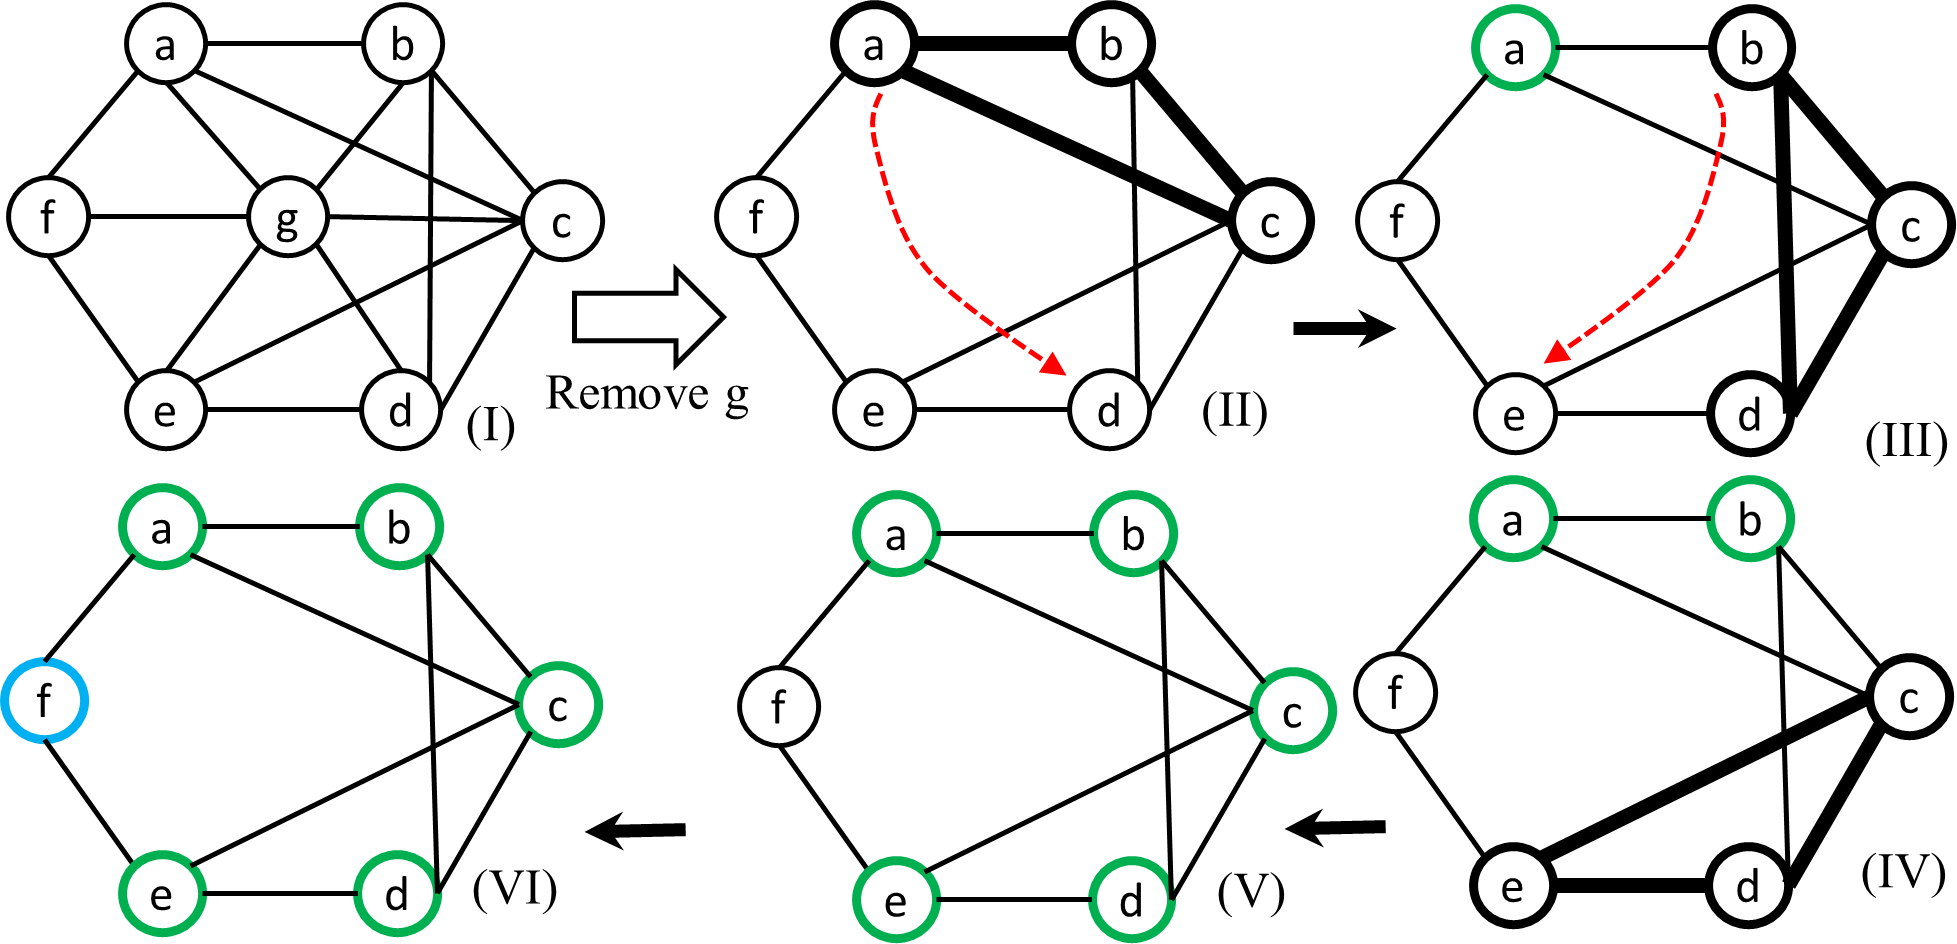
\includegraphics[width=\columnwidth]{./texfiles/Chapter_2/figures/percolation}
\caption{Illustrative example of 3-clique percolation. Once node $g$ is removed, a 3-clique is placed on node $a$. The clique  percolates and accumulates all the nodes except node $f$ which forms a singleton community along with $\{a,b,c,d,e\}$.}\label{fig_percolation} 
%\vspace{-3mm}
\end{figure}

\noindent$\bullet$ \underline{Adjust communities after removing a node:} When $G_s$ is full, we remove $m$ nodes (and their adjacent edges) from the sample using $CheckResizeSample()$ (Function 7). Since each such node $u$ is already a part of its community $C(u)$, its deletion might keep the previous community structure unchanged, or break the community into smaller parts, or merge several communities together. The community structure $C_s$ is adjusted using  $CommunityAfterNodeRemoval()$ (Function 8) incrementally.  Let us consider two extreme cases -- a node with degree $1$ is removed, and a node with highest degree is removed. Removal of a single degree node will keep the community unchanged. However, removal of a highest degree node can render the community disconnected or broken into smaller parts which might further merge to the other existing communities. Here we utilize the clique percolation method \cite{PalEtAl05} to handle this situation efficiently. In particular, when a vertex $v$ is removed from a community $C$, we place a 3-clique to one of its neighbors and let the clique percolate until no vertices in $C$ are discovered. Nodes discovered in each such clique percolation will form a community. We repeat this clique percolation from each of $v$'s neighbors until each member in $C$ is assigned to a community. For example, in Figure \ref{fig_percolation} when node $g$ is removed, we place a 3-clique on its neighbor $a$. Once the 3-clique starts percolating, it accumulates all nodes except $f$. Therefore, two new communities $\{a,b,c,d,e\}$ and $\{f\}$  emerge due to the deletion of $g$. In this way, we let the remaining communities of $C$ choose their best communities to merge in.% \TODO{It is not clear how you make a community merge into the best possible candidate. In fact, this part is extremely hard to follow. More detailed and explanatory writing + a figure to illustrate the situation is needed {\color{blue} Done}}.
\begin{function7}
\caption{$CheckResizeSample(V_s,C_s,n,m)$}
\If{$V_s == n$}{
Remove $m$ nodes say, $u_1, u_2,\cdots, u_m$  (and all their adjacent edges) from $G_s$ having lowest degree\\
\For{$u\in \{u_1,u_2,\cdots,u_m\}$}{
$C_s \leftarrow CommunityAfterNodeRemoval(u,C_s)$
}
}
\Return $V_s,E_s,C_s$
\end{function7}

%\vspace{-8mm}

\begin{function8}
\caption{$CommunityAfterNodeRemoval(u,C_s)$}
Assume node $u$ and its adjacent edges are removed from $G_s$\\
$i=1$\\
\While{$N(u)\neq \phi$}{
$b_i$=Nodes found by a 3-clique percolation on $v\in N(u)$\\
\If{$b_i==\phi$}{
$b_i=\{v\}$
}
$C_s=C_s \cup b_i$\\
$N(u)=N(u)\setminus b_i$\\
$i=i+1$\\
}
%Let each singleton in $N(a)$ consider its best communities \TODO{Not clear how this is done?}\\
%Let each $b_i$ consider its best communities \TODO{Not clear how this is done?}\\
Update $C_i$\\% \TODO{What does this line do?}\\
\Return $C_s$   
\end{function8}


%{\color{red}
%1. When blindly enter the edges, do we increase the counter.\\
%2. Assume that $G_s$ can take only one node. If you try to add $u,v$ together, what would happen\\
%3. No edge deletion case in your algorithm\\
%4. In case of BothNew, if buffer has only one vacant place, what would happen. For me, we should add $u$ and $v$ one by one and follow the previous step, instead of adding together,
%}
